\documentclass[12pt,a4paper]{article}
\usepackage[utf8]{vietnam}
\usepackage{amsmath,amssymb}
\usepackage{tabularx}
\usepackage{tikz}
\usetikzlibrary{calc,angles,quotes,arrows.meta,patterns}
\usepackage{xcolor}
\usepackage{enumitem}
\usepackage{fancyhdr}
\usepackage{graphicx}
\usepackage[top=0.9cm, bottom=0.9cm, left=1.2cm, right=1.2cm]{geometry}
\usepackage[loigiai]{ex_test}
\SAOPTN{widthSA=3.2,heightSA=0.62}

\setlength{\headheight}{15pt}
\setlength{\parskip}{0pt}

\pagestyle{fancy}
\fancyhf{}
\rhead{\textit{Môn Toán 8 -- Hướng dẫn giải Đề số 05}}
\lhead{\textit{Bộ đề ôn tập Giữa học kì I}}
\cfoot{\thepage}

\begin{document}

\begin{center}
  \textbf{\Large HƯỚNG DẪN GIẢI CHI TIẾT VÀ BẢNG ĐÁP ÁN}\\
  \textbf{\large ĐỀ ÔN TẬP GIỮA HỌC KỲ I -- ĐỀ SỐ 05}\\
  \textit{Môn: Toán 8 -- Năm học 2026 -- 2027}
\end{center}
\vspace{2mm}

% --- BẢNG ĐÁP ÁN TRẮC NGHIỆM TÓM TẮT ---
\noindent\textbf{\large A. BẢNG ĐÁP ÁN TRẮC NGHIỆM TỔNG HỢP}
\vspace{1mm}

\noindent\textbf{1. Phần I (Mỗi câu trả lời đúng được 0,25 điểm):}
\begin{center}
\begin{tabular}{|c|c|c|c|c|c|c|c|c|c|c|c|c|}
\hline
\textbf{Câu} & \textbf{1} & \textbf{2} & \textbf{3} & \textbf{4} & \textbf{5} & \textbf{6} & \textbf{7} & \textbf{8} & \textbf{9} & \textbf{10} & \textbf{11} & \textbf{12} \\
\hline
\textbf{Đ/A} & \textbf{A} & \textbf{B} & \textbf{C} & \textbf{D} & \textbf{D} & \textbf{A} & \textbf{B} & \textbf{D} & \textbf{D} & \textbf{B} & \textbf{A} & \textbf{A} \\
\hline
\end{tabular}
\end{center}
\vspace{0.5mm}

\noindent\textbf{2. Phần II (Đúng 1 ý: 0,1đ; 2 ý: 0,25đ; 3 ý: 0,5đ; 4 ý: 1,0đ):}
\begin{center}
\begin{tabular}{|c|c|c|c|c||c|c|c|c|c|}
\hline
\textbf{Câu} & \textbf{a)} & \textbf{b)} & \textbf{c)} & \textbf{d)} & \textbf{Câu} & \textbf{a)} & \textbf{b)} & \textbf{c)} & \textbf{d)} \\
\hline
\textbf{Câu 1} & \textbf{Đ} & \textbf{Đ} & \textbf{Đ} & \textbf{S} & \textbf{Câu 2} & \textbf{Đ} & \textbf{Đ} & \textbf{Đ} & \textbf{S} \\
\hline
\end{tabular}
\end{center}
\vspace{0.5mm}

\noindent\textbf{3. Phần III (Mỗi câu trả lời đúng được 1,0 điểm):}
\begin{center}
\begin{tabular}{|c|c|c|}
\hline
\textbf{Câu} & \textbf{Câu 1} & \textbf{Câu 2} \\
\hline
\textbf{Đáp án} & $\mathbf{x = \dfrac{10}{7}}$ & $\mathbf{75^\circ}$ \\
\hline
\end{tabular}
\end{center}
\vspace{1.5mm}

% --- B. LỜI GIẢI CHI TIẾT ---
\noindent\textbf{\large B. LỜI GIẢI CHI TIẾT CÁC CÂU HỎI}
\vspace{1mm}
\begin{ex}
Trong các biểu thức sau, biểu thức nào không là đa thức?
\choice
{\True $\dfrac{5}{xy}$}
{$12x^2y$}
{$5$}
{$x^2y + 3xy + 1$}
\loigiai{
Biểu thức $\dfrac{5}{xy}$ có chứa biến ở mẫu số nên không phải là đa thức.
}
\end{ex}

\begin{ex}
Trong các đơn thức sau, đơn thức nào đồng dạng với đơn thức $-\dfrac{3}{4}x^2y^3$?
\choice
{$-\dfrac{3}{4}x^3y^2$}
{\True $y^3x^2$}
{$2xy$}
{$3x^2y^3z$}
\loigiai{
Hai đơn thức đồng dạng là hai đơn thức có hệ số khác 0 và có cùng phần biến. Đơn thức $y^3x^2 = x^2y^3$ có cùng phần biến với đơn thức đã cho.
}
\end{ex}

\begin{ex}
Đơn thức $10x^3y^2z^3$ chia hết cho đơn thức nào sau đây?
\choice
{$5x^3y^3z^2$}
{$-2x^4y^2z$}
{\True $-9x^3yz^2$}
{$2x^3y^3z^3$}
\loigiai{
Xét đơn thức $-9x^3yz^2$, số mũ của các biến $x, y, z$ lần lượt là $3, 1, 2$ đều nhỏ hơn hoặc bằng số mũ tương ứng trong $10x^3y^2z^3$ (lần lượt là $3, 2, 3$). Do đó $10x^3y^2z^3$ chia hết cho $-9x^3yz^2$.
}
\end{ex}

\begin{ex}
Kết quả phép tính $2x(x - 2y)$ bằng:
\choice
{$2x^2 - 2y^2$}
{$2x^2 - 4y^2$}
{$2x^2 - 2xy$}
{\True $2x^2 - 4xy$}
\loigiai{
Thực hiện nhân đơn thức với đa thức: $2x(x - 2y) = 2x \cdot x - 2x \cdot 2y = 2x^2 - 4xy$.
}
\end{ex}

\begin{ex}
Kết quả phép tính $(x - 2y)(x + 2y)$ bằng:
\choice
{$x^2 - 2y^2$}
{$(x + 2y)^2$}
{$(x - 2y)^2$}
{\True $x^2 - 4y^2$}
\loigiai{
Áp dụng hằng đẳng thức hiệu hai bình phương: $(x - 2y)(x + 2y) = x^2 - (2y)^2 = x^2 - 4y^2$.
}
\end{ex}

\begin{ex}
Đa thức $4x^2 - 9$ được phân tích thành nhân tử là:
\choice
{\True $(2x - 3)(2x + 3)$}
{$(4x + 9)(4x - 9)$}
{$(4x - 3)(4x + 3)$}
{$(2x + 9)(2x - 9)$}
\loigiai{
Biến đổi biểu thức về dạng hiệu hai bình phương: $4x^2 - 9 = (2x)^2 - 3^2 = (2x - 3)(2x + 3)$.
}
\end{ex}

\begin{ex}
Giá trị của biểu thức $x^2 - 2xy + y^2 - 3$ tại $x = -1, y = 2$ là:
\choice
{$-6$}
{\True $6$}
{$12$}
{$-12$}
\loigiai{
Thu gọn biểu thức: $x^2 - 2xy + y^2 - 3 = (x - y)^2 - 3$. Thay $x = -1, y = 2$: $(-1 - 2)^2 - 3 = (-3)^2 - 3 = 9 - 3 = 6$.
}
\end{ex}

\begin{ex}
Tổng số đo các góc trong một tứ giác bằng:
\choice
{$90^\circ$}
{$120^\circ$}
{$180^\circ$}
{\True $360^\circ$}
\loigiai{
Theo định lý về tổng các góc của một tứ giác, tổng số đo 4 góc luôn bằng $360^\circ$.
}
\end{ex}

\begin{ex}
Tứ giác $ABCD$ là hình bình hành nếu:
\choice
{$\widehat{A} = \widehat{C}$}
{$\widehat{B} = \widehat{D}$}
{$AB \parallel CD$, $AB = AD$}
{\True $\widehat{A} = \widehat{C}$ và $\widehat{B} = \widehat{D}$}
\loigiai{
Dấu hiệu nhận biết hình bình hành: tứ giác có các góc đối bằng nhau là hình bình hành, tức là $\widehat{A} = \widehat{C}$ và $\widehat{B} = \widehat{D}$.
}
\end{ex}

\begin{ex}
Độ dài cạnh hình thoi có hai đường chéo bằng $6\text{ cm}$ và $8\text{ cm}$ là:
\choice
{$21\text{ cm}$}
{\True $5\text{ cm}$}
{$14\text{ cm}$}
{$\sqrt{11}\text{ cm}$}
\loigiai{
Hai đường chéo của hình thoi vuông góc và cắt nhau tại trung điểm. Nửa độ dài hai đường chéo là $3\text{ cm}$ và $4\text{ cm}$. Áp dụng định lý Pythagore: $a = \sqrt{3^2 + 4^2} = 5\text{ cm}$.
}
\end{ex}

\begin{ex}
Cho hình chóp tam giác đều có diện tích đáy bằng $12\text{ cm}^2$ và chiều cao bằng $5\text{ cm}$. Thể tích của hình chóp đó là:
\choice
{\True $20\text{ cm}^3$}
{$60\text{ cm}^3$}
{$15\text{ cm}^3$}
{$30\text{ cm}^3$}
\loigiai{
Thể tích hình chóp là: $V = \dfrac{1}{3} S \cdot h = \dfrac{1}{3} \cdot 12 \cdot 5 = 20\text{ cm}^3$.
}
\end{ex}

\begin{ex}
Kết quả phân tích đa thức $x^3 + 8$ thành nhân tử là:
\choice
{\True $(x + 2)(x^2 - 2x + 4)$}
{$(x + 2)(x^2 + 2x + 4)$}
{$(x - 2)(x^2 + 2x + 4)$}
{$(x + 2)^3$}
\loigiai{
Áp dụng hằng đẳng thức tổng hai lập phương: $x^3 + 8 = x^3 + 2^3 = (x + 2)(x^2 - 2x + 4)$.
}
\end{ex}


\setcounter{ex}{0}
\noindent\textbf{\large PHẦN II. CÂU TRẮC NGHIỆM ĐÚNG SAI}
\vspace{1mm}
\begin{ex}
Cho biểu thức $P = \left(\dfrac{1}{x - 2} - \dfrac{1}{x + 2}\right) \cdot \dfrac{x^2 - 4}{4}$ với $x \neq \pm 2$. Xét tính đúng sai của các mệnh đề sau:
\choiceTF
{\True Mẫu thức chung của hai phân thức trong ngoặc là $x^2 - 4$}
{\True Kết quả rút gọn biểu thức trong ngoặc là $\dfrac{4}{x^2 - 4}$}
{\True Giá trị của biểu thức $P$ sau khi rút gọn bằng $1$}
{Tại $x = 3$, giá trị của biểu thức $P$ bằng $3$}
\loigiai{
\textbf{a)} \textbf{Đúng.} Mẫu thức chung là $(x - 2)(x + 2) = x^2 - 4$.

\textbf{b)} \textbf{Đúng.} Ta có: $\dfrac{1}{x - 2} - \dfrac{1}{x + 2} = \dfrac{(x + 2) - (x - 2)}{x^2 - 4} = \dfrac{4}{x^2 - 4}$.

\textbf{c)} \textbf{Đúng.} $P = \dfrac{4}{x^2 - 4} \cdot \dfrac{x^2 - 4}{4} = 1$.

\textbf{d)} \textbf{Sai.} Với mọi $x \neq \pm 2$, $P = 1$ luôn không đổi. Do đó tại $x = 3$ thì $P = 1 \neq 3$.
}
\end{ex}

\begin{ex}
Cho phương trình $(x - 3)(x + 3) - x(x - 2) = 5$. Xét tính đúng sai của các mệnh đề sau:
\choiceTF
{\True Khai triển tích $(x - 3)(x + 3)$ ta được $x^2 - 9$}
{\True Biến đổi vế trái của phương trình ta được $2x - 9$}
{\True Phương trình có nghiệm duy nhất $x = 7$}
{Nghiệm $x = 7$ không là nghiệm của phương trình $3x - 5 = 16$}
\loigiai{
\textbf{a)} \textbf{Đúng.} Áp dụng hằng đẳng thức hiệu hai bình phương: $(x - 3)(x + 3) = x^2 - 9$.

\textbf{b)} \textbf{Đúng.} Ta có: $(x^2 - 9) - (x^2 - 2x) = x^2 - 9 - x^2 + 2x = 2x - 9$.

\textbf{c)} \textbf{Đúng.} Phương trình tương đương $2x - 9 = 5 \Leftrightarrow 2x = 14 \Leftrightarrow x = 7$.

\textbf{d)} \textbf{Sai.} Thay $x = 7$ vào: $3 \cdot 7 - 5 = 21 - 5 = 16$, do đó $x = 7$ là nghiệm của phương trình $3x - 5 = 16$.
}
\end{ex}


\setcounter{ex}{0}
\noindent\textbf{\large PHẦN III. CÂU HỎI TRẢ LỜI NGẮN}
\vspace{1mm}
\begin{ex}
Tìm $x$, biết: $(x + 2)^2 - x(x - 3) = 14$. \shortans{$x = \dfrac{10}{7}$}
\loigiai{
Ta có:
$(x^2 + 4x + 4) - (x^2 - 3x) = 14$

$\Leftrightarrow x^2 + 4x + 4 - x^2 + 3x = 14$

$\Leftrightarrow 7x + 4 = 14$

$\Leftrightarrow 7x = 10 \Leftrightarrow x = \dfrac{10}{7}$.
}
\end{ex}

\begin{ex}
Cho hình thang cân $ABCD$ có $\widehat{A} = 105^\circ$. Tính số đo góc $\widehat{C}$? \shortans{$75^\circ$}
\loigiai{
Vì $AB \parallel CD$ nên hai góc trong cùng phía bù nhau:
$\widehat{D} = 180^\circ - \widehat{A} = 180^\circ - 105^\circ = 75^\circ$.

Vì $ABCD$ là hình thang cân nên hai góc kề một đáy bằng nhau, do đó: $\widehat{C} = \widehat{D} = 75^\circ$.
}
\end{ex}


\setcounter{ex}{0}
\noindent\textbf{\large PHẦN IV. TỰ LUẬN (HƯỚNG DẪN GIẢI VÀ THANG ĐIỂM)}
\vspace{1mm}
\begin{ex} (1,0 điểm)
Thực hiện phép tính (rút gọn nếu có thể):
\begin{enumerate}[label=\textbf{\alph*)}, leftmargin=0.8cm, itemsep=0pt, topsep=1pt]
\item (0,35 điểm) $(2x^2 + 3xy) + (x^2 - xy)$
\item (0,35 điểm) $(2x + y)(x - 3y)$
\item (0,3 điểm) $(9x^2y^3 - 6x^3y^2 + 4x^2y^2) : (3x^2y)$
\end{enumerate}
\loigiai{
\textbf{a)} \textit (0,35 điểm): Ta có: $(2x^2 + 3xy) + (x^2 - xy) = (2x^2 + x^2) + (3xy - xy) = 3x^2 + 2xy$.

\textbf{b)} \textit (0,35 điểm): Ta có: $(2x + y)(x - 3y) = 2x^2 - 6xy + xy - 3y^2 = 2x^2 - 5xy - 3y^2$.

\textbf{c)} \textit (0,3 điểm): Ta có: $(9x^2y^3 - 6x^3y^2 + 4x^2y^2) : (3x^2y) = 9x^2y^3 : 3x^2y - 6x^3y^2 : 3x^2y + 4x^2y^2 : 3x^2y = 3y^2 - 2xy + \dfrac{4}{3}y$.


}
\end{ex}
\vspace{0.5mm}

\begin{ex} (0,75 điểm)
Cho hai đa thức: $A = x^7 - 4x^3y^2 - 5xy + 7$ và $B = x^7 + 5x^3y^2 - 3xy - 3$.
\begin{enumerate}[label=\textbf{\alph*)}, leftmargin=0.8cm, itemsep=0pt, topsep=1pt]
\item (0,4 điểm) Tìm đa thức $C$ sao cho $C = A + B$.
\item (0,35 điểm) Tìm đa thức $D$ sao cho $A + D = B$.
\end{enumerate}
\loigiai{
\textbf{a)} \textit (0,4 điểm): $C = (x^7 - 4x^3y^2 - 5xy + 7) + (x^7 + 5x^3y^2 - 3xy - 3) = (x^7 + x^7) + (-4x^3y^2 + 5x^3y^2) + (-5xy - 3xy) + (7 - 3) = 2x^7 + x^3y^2 - 8xy + 4$.

\textbf{b)} \textit (0,35 điểm): Từ $A + D = B \Rightarrow D = B - A$.
$D = (x^7 + 5x^3y^2 - 3xy - 3) - (x^7 - 4x^3y^2 - 5xy + 7) = (x^7 - x^7) + (5x^3y^2 + 4x^3y^2) + (-3xy + 5xy) + (-3 - 7) = 9x^3y^2 + 2xy - 10$.


}
\end{ex}
\vspace{0.5mm}

\begin{ex} (0,75 điểm)
Cho tam giác $ABC$ vuông cân tại $A$, đường trung tuyến $AM$. Gọi $N$ là trung điểm của $AC$. Vẽ điểm $D$ đối xứng với điểm $M$ qua $N$.
\begin{center}
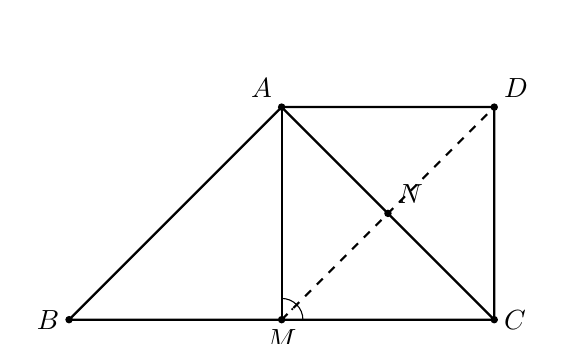
\begin{tikzpicture}[scale=0.9, >=stealth]
  \coordinate (A) at (0,3);
  \coordinate (B) at (-3,0);
  \coordinate (C) at (3,0);
  \coordinate (M) at (0,0);
  \coordinate (N) at ($(A)!0.5!(C)$);
  \coordinate (D) at ($(N)!-1!(M)$);
  \draw[thick] (A)--(B)--(C)--cycle;
  \draw[thick] (A)--(M);
  \draw[thick] (A)--(D)--(C);
  \draw[thick, dashed] (M)--(D);
  \fill (A) circle (1.5pt) node[above left] {$A$};
  \fill (B) circle (1.5pt) node[left] {$B$};
  \fill (C) circle (1.5pt) node[right] {$C$};
  \fill (M) circle (1.5pt) node[below] {$M$};
  \fill (N) circle (1.5pt) node[above right] {$N$};
  \fill (D) circle (1.5pt) node[above right] {$D$};
  \draw (0.3,0) arc (0:90:0.3);
  \fill (0.15,0.15) circle (0.5pt);
\end{tikzpicture}
\end{center}
\begin{enumerate}[label=\textbf{\alph*)}, leftmargin=0.8cm, itemsep=0pt, topsep=1pt]
\item (0,35 điểm) Chứng minh $AM = MC$.
\item (0,4 điểm) Chứng minh tứ giác $ADCM$ là hình vuông.
\end{enumerate}
\loigiai{
\textbf{a)} \textit (0,35 điểm): Trong tam giác $ABC$ vuông tại $A$, đường trung tuyến $AM$ ứng với cạnh huyền $BC$ có độ dài bằng nửa cạnh huyền: $AM = \dfrac{1}{2}BC = MC$.

\textbf{b)} \textit (0,4 điểm): Tứ giác $ADCM$ có hai đường chéo $AC$ và $MD$ cắt nhau tại trung điểm $N$ của mỗi đường, do đó $ADCM$ là hình bình hành.

Hình bình hành $ADCM$ có $AM = MC$ nên là hình thoi.

Tam giác $ABC$ cân tại $A$ có $AM$ là trung tuyến đồng thời là đường cao nên $AM \perp BC$, tức là $\widehat{AMC} = 90^\circ$.

Hình thoi $ADCM$ có một góc vuông ($\widehat{AMC} = 90^\circ$) nên $ADCM$ là hình vuông.


}
\end{ex}
\vspace{0.5mm}

\begin{ex} (0,5 điểm)
Tìm giá trị nhỏ nhất của biểu thức: $M = 9x^2 + 6y^2 + 18x - 12xy - 12y - 27$.
\begin{enumerate}[label=\textbf{\alph*)}, leftmargin=0.8cm, itemsep=0pt, topsep=1pt]
\item (0,5 điểm) Tìm giá trị nhỏ nhất của $M$.
\end{enumerate}
\loigiai{
\textbf{a)} \textit (0,5 điểm): Biến đổi biểu thức $M$:

$M = (9x^2 - 12xy + 4y^2 + 18x - 12y + 9) + 2y^2 - 36$

$= [(3x - 2y)^2 + 2 \cdot (3x - 2y) \cdot 3 + 3^2] + 2y^2 - 36$

$= (3x - 2y + 3)^2 + 2y^2 - 36$.

Vì $(3x - 2y + 3)^2 \ge 0$ và $2y^2 \ge 0$ với mọi $x, y$, nên $M \ge -36$.

Dấu "=" xảy ra khi và chỉ khi: $\begin{cases} 2y^2 = 0 \\ 3x - 2y + 3 = 0 \end{cases} \Leftrightarrow \begin{cases} y = 0 \\ x = -1 \end{cases}$.

Vậy giá trị nhỏ nhất của $M$ là $-36$, đạt được khi $x = -1$ và $y = 0$.


}
\end{ex}
\vspace{0.5mm}


\enlargethispage{1.5cm}
\begin{center}
\rule{4cm}{0.4pt}\\
\textit{--- HẾT ---}
\end{center}
\end{document}
